\documentclass[12pt,titlepage]{article}
\setlength{\headheight}{14.5pt}
\addtolength{\topmargin}{-2.5pt}
 
\usepackage{cite}

\usepackage{pgfplots} % Add this line to include the pgfplots package
 \usepackage{amsmath}
\usepackage{geometry}
\usepackage{setspace}
\usepackage{graphicx}
\usepackage{fancyhdr}
\usepackage{xcolor}
\usepackage{titlesec}
\usepackage{booktabs}
\usepackage{hyperref}
\usepackage{soul}
\usepackage{wrapfig}
\usepackage{placeins}
\usepackage{float}
\usepackage{amsmath}
\usepackage{caption}
%\usepackage[style=numeric,sorting=none]{biblatex}
%\addbibresource{references.bib}


\hypersetup{
    colorlinks=true,       % Enable colored links
    linkcolor=black,       % Color of internal links
    filecolor=black,       % Color of file links
    urlcolor=black,        % Color of external links
    citecolor=black        % Color of citation links
}


\renewcommand{\headrulewidth}{0pt} % Remove header rule
\renewcommand{\footrulewidth}{0pt} % Remove footer rule




\usepackage{url}
\geometry{a4paper, margin=0.7in }
\setlength{\parindent}{0pt}
\setstretch{1.5}
\headsep = 5pt %Move text closer to header
\usepackage{setspace}
% Header and Footer
\usepackage{fancyhdr}
\pagestyle{fancy}
\fancyhf{} % Clear all header and footer fields
\fancyhead[L]{\textbf{19-AIBM4}} % Top-left text

\renewcommand{\headrule}{\vspace{1pt}\hrule height 0.5pt} %Headrule spacing

% Optional: Adjust header line thickness if needed
\renewcommand{\headrulewidth}{0.5pt} % Thickness of the header line

% Combine the page numbering and horizontal rule into one footer definition
\fancyfoot[C]{\rule{\textwidth}{0.5pt}\\ Page \thepage\ of 15} % Bottom horizontal line with page number


% Title formatting
\titleformat{\section}[block]
  {\large\bfseries\sffamily\color{black}}
  {\thesection.}{1em}{}


\titleformat{\subsection}[block]
  {\normalsize\bfseries\sffamily\color{black}}
  {\thesubsection}{1em}{}
 \pgfplotsset{compat=1.18} 

 \titlespacing*{\subsection}{0pt}{1em}{0.2em}
 \titlespacing*{\section}{0pt}{1em}{0.5em}
\linespread{1.5}
\setlength{\abovedisplayskip}{0pt}
\setlength{\belowdisplayskip}{0pt}



\begin{document}


\pagenumbering{arabic} % Ensure Arabic numbering starts from the first page



 
% -------------------------------------------------------------
% COVER PAGE
% -------------------------------------------------------------
\begin{titlepage}
\centering
% University logo or other image
\includegraphics[width=0.4\textwidth]{UoD_Engineering.jpg} \\
\vspace{10mm}

% Title and subtitle
{\LARGE \textbf{Feasibility Report for Group 19-AIBM4 Autonomous Material Mover}} \\[10pt]

\vspace{5mm}\hrule\vspace{0mm}

% Insert image with caption for the material mover
\begin{figure}[h!]
    \centering
     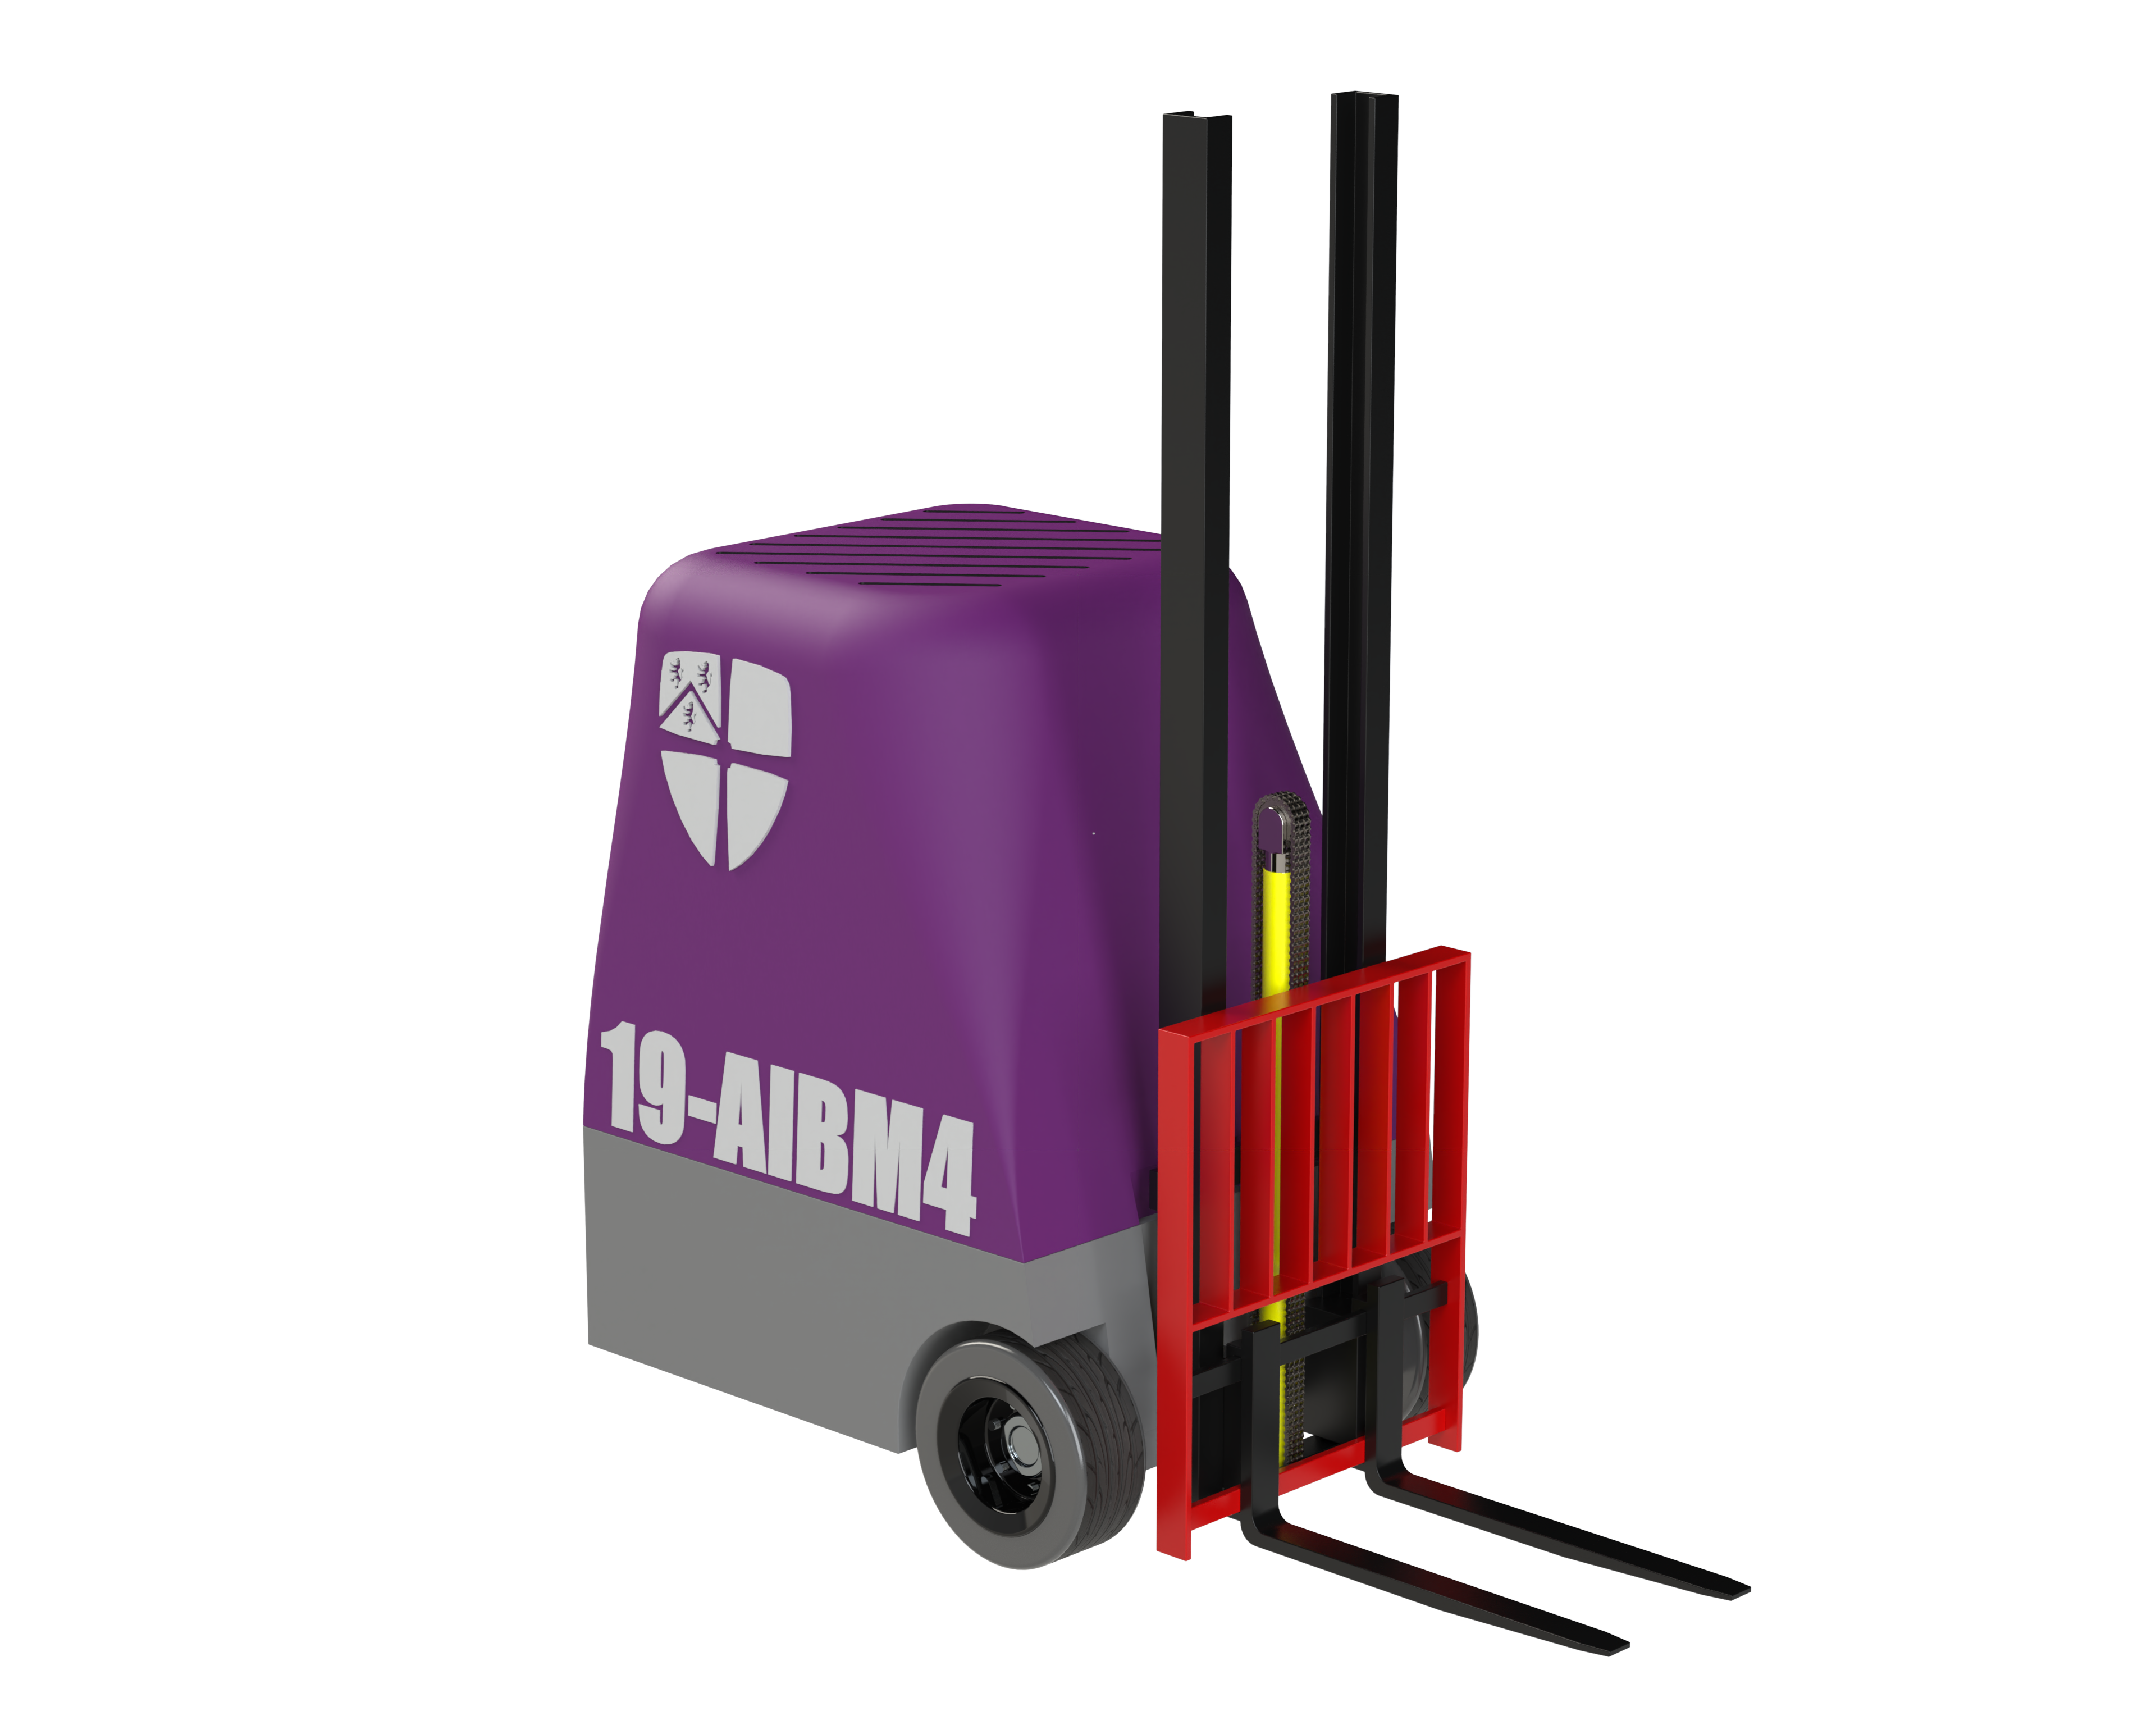
\includegraphics[width=1\textwidth]{Initial Final (7).png}
\end{figure}  
\vspace{0mm}
\vspace{10mm}

% Title and author block
{\large \textbf{Co-Authors: }\textit{A Wright, A Wigmore, H Billing, J Wang, L Nangle, \newline W Woodward}} \\ \vspace{1mm}
{Supervisors:\textit{ Dr Aissa Ikhlef, Mr Bill Maxwell}} \\[10pt]
{\small Durham University \\ \today}
\end{titlepage}
\addtocounter{page}{1}

\section*{Executive Summary}

This feasibility report looks into the development of an Automated Material Mover (AIBM4), which aims to transport materials autonomously within a factory environment. This would eliminate the need for manual handling of goods, improve productivity and ensure a safer and more sustainable working environment. 
\par Through an iterative design process, we chose a three-wheeled automated forklift design that integrates differential steering around a central axle for maximum manoeuvrability and tape sensing technology for precise movement within a factory environment. To make this design contemporary and sustainable, the body and forks will be made out of steel due to its high reconcilability and we will use airless tyres to improve durability and reduce waste.
\par Engineering calculations validate the design's structural integrity and feasibility as well as ensuring compliance with ISO 3691-4  standards. An in-depth cost analysis demonstrates that automated guided vehicles (AGVs) are financially viable over conventional manual forklifts, due to significant savings in labour and operating costs over time. 
\par An adaptable factory layout design has been included which has been optimised for AGV operation, however the material mover has been designed to fit into the majority of modern-day factories. We have also conducted a risk assessment to mitigate any risks as well as created a Gantt chart which determines that the design process will be finished by the end of March 2025.
\par This report demonstrates the technical, economic and environmental upper hand that an automated material mover can provide in a modern factory setting.

\vspace{2em}

% -------------------------------------------------------------
% FRONTMATTER
% -------------------------------------------------------------
\tableofcontents
%\begin{figure}[h!]
 %   \centering
 %    \includegraphics[width=0.65\textwidth]{finaldesign.png}
 %         \label{fig:final design}
%\end{figure}

% -------------------------------------------------------------
% MAIN CONTENT
% -------------------------------------------------------------


% -------------------------------------------------------------
% 2. Introduction and Project Scope
% -------------------------------------------------------------

\vspace{2em}

\section{Introduction}
\subsection{What is the problem that we are attempting to solve?}
Efficient material handling is essential in modern manufacturing, but conventional forklifts still require manual operation. This project seeks to eliminate manual dependency by designing an autonomous material mover.
 
\subsection{Issues with Conventional Manual Material Handling}

Manual labour and forklifts have several key issues within factory environments:

\begin{itemize}
    \item \textbf{Inefficiency:} Human workers require regular breaks, reducing productivity.
    \item \textbf{Safety concerns:} Human error can lead to an increased likelihood of an accident as well as a higher chance of injuries.
    \item \textbf{Cost:} Cost of labour is very large, and multiple shifts necessitates additional hiring costs.
    \item \textbf{Reliability:} Human error can lead to materials being moved to the wrong locations.
\end{itemize}

Overall, these issues reduce productivity and compromise workplace safety.


\section{Project Scope}
\FloatBarrier
\vspace{-20pt}
\begin{figure}[H]
    \centering
    \includegraphics[width=1\linewidth]{ScopeCanvas1.png}
\end{figure}
\vspace{-3em}
\begin{figure}[H]
    \centering
    \includegraphics[width=1\linewidth]{ScopeCanvas2.png}
\end{figure}
\vspace{-40pt}
\begin{figure}[H]
     \centering
    \includegraphics[width=1\linewidth]{ScopeCanvas3.png}
 \end{figure}
 \vspace{-3em}
\begin{figure}[H]
     \centering
    \includegraphics[width=1\linewidth]{Scope Canvas 4.png}
    \vspace{-30pt}
    \caption{Scope Canvas}
     \label{fig:Scope Canvas}
\end{figure}
\FloatBarrier
\vspace{-20pt}
\section{User-Requirement-Specification}
\vspace{-20pt}
\begin{figure}[htbp]
    \centering
    \includegraphics[width=1\textwidth]{URS1.png}
    \vspace{-20pt}
    \caption{URS – Automated Material Mover Project}
    \label{fig:URS}
\end{figure}

\FloatBarrier

\vspace{-20pt}


% -------------------------------------------------------------
% 3. Concepts
% -------------------------------------------------------------
\section{Concepts}

\subsection{Initial Concepts}
 
\begin{enumerate}
     \item A three-wheeled mover with magnetic tape sensors. This design utilises a compact three wheeled configuration to allow for maximum manoeuvrability in tight spaces. Due to its magnetic tape sensing technology it can accurately navigate predefined paths within a factory setting and be easily integrated and changed within factories.
    \item A four-wheeled mover on a monorail. This design uses a monorail to ensure extremely precise movement as well as a four wheel base which makes it very sturdy for lifting goods and transporting them quickly and efficiently. An advantage of the design was that there was no down-time due to the material mover being constantly connected to a power source.
    \item A six-wheeled mover with line-following sensors. Six wheels allows for superior stability and load-bearing capabilities as well as maximum manoeuvrability. It would use differential steering for its central axis, with the other four wheels being caster wheels, to allow it to spin on the spot making it highly manoeuvrable and versatile.
 \end{enumerate}

 
\vspace{-20pt}
\begin{figure}[H]
    \centering
    \begin{minipage}{0.32\textwidth}
        \centering
        \includegraphics[width=\textwidth]{Simple_sketch_of_an_automated_forklift_robot_with_two_wheels_at_the_back_and_one_wheel_in_the_front.png}
        \caption{\raggedright Concept 1: Three-wheel magnetic tape following design}
    \end{minipage}%
    \hspace{0.01\textwidth}
    \begin{minipage}{0.32\textwidth}
        \centering
        \includegraphics[width=\textwidth]{Concept2.png}
        \caption{\raggedright Concept 2: Four-wheel monorail design}
    \end{minipage}%
    \hspace{0.01\textwidth}
    \begin{minipage}{0.32\textwidth}
        \centering
        \includegraphics[width=\textwidth]{Louis' design without text.png}
        \vspace{0.34em}
        \caption{\raggedright Concept 3: Six-wheel line following design}
    \end{minipage}
\end{figure}

\vspace{-28pt}
 

\subsection{Strengths and Weaknesses}
\vspace{-5pt}
Each concept was evaluated against the URS using a design decision matrix. A summary of this is provided in Table \ref{tab:concept_evaluation} below.

\vspace{-10pt}
\begin{table}[h!]
\centering
\caption{Concept Evaluation Matrix}
\begin{tabular}{@{}lccc@{}}
\toprule
\textbf{Criteria}      & \textbf{Concept 1} & \textbf{Concept 2} &\textbf{Concept 3} \\ \midrule
Load Capacity          & High               & Medium              & Medium            \\
Navigation Efficiency  & Medium             & High                & High              \\
Cost                   & Low                & Medium              & Medium            \\
Ease of Maintenance    & High               & Low                 & Low               \\ \bottomrule
\end{tabular}
\label{tab:concept_evaluation}
\end{table}
\FloatBarrier


\vspace{-25pt}
\section{Chosen Solution}
\vspace{-20pt}
\begin{figure}[ht]
    \centering
    \begin{minipage}[t]{0.52\textwidth}
    \vspace{0pt}
    \setstretch{1.2}
        Initially, the pooling of design ideas resulted in Figure 6. However,
        it was then decided that the lifter ought to pick items off the floor, leading to a redesign resulting in the counterbalance forklift in figure 7. The wheels were placed in a tadpole configuration to give better manoeuvrability and dynamic stability. The vehicle will be guided by magnetic tape on the factory floor detected by sensors on the undercarriage. The forks make use of a hydraulic lifting system, and will be charged using a wireless charging system which is adjacent to the main path.
    \end{minipage}%
    \hfill
    \begin{minipage}[t]{0.22\textwidth}
        \vspace{10pt} 
        \centering
        \includegraphics[width=\linewidth]{Initial Pooled (4) Cropped.png}  
        %\vspace{-15pt}
        \captionsetup{width=0.8\textwidth}
        \caption{Initial Pooled Design}
        \label{fig:x}
    \end{minipage}
    \begin{minipage}[t]{0.22\textwidth}
        \vspace{-2pt} 
        \centering
        \includegraphics[width=\linewidth]{Initial Final (7) Cropped.png}  
        %\vspace{-15pt}
        \captionsetup{width=0.7\textwidth}
        \caption{Final Design}
        \label{fig:x}
    \end{minipage}
\end{figure}
\FloatBarrier


\FloatBarrier

\subsection{Sustainability}
In order to make the design sustainable, the body and forks are likely to be made from steel because it has the highest recycling rate among all materials used in construction and engineering \cite{baker2023}. The castor wheels can be made of high-quality pre-consumer nylon (from the waste of polyester production) \cite{eco2022} and the drive wheels can be airless tires, as this would reduce the amount of rubber that goes into landfill and improve fuel efficiency \cite{ImperialTyres}. For lithium-ion batteries, a hydrometallurgical process can be used, where 80\% of the battery can be recycled and 95\% of the valuable materials can be recovered and used for new batteries \cite{Lithium-ion}.

\subsection {Engineering Calculations}
\vspace{-8pt}
\begin{figure}[H]
    \centering
    \begin{minipage}[t]{0.5\textwidth}
        \vspace{0pt}
        \linespread{1.5}
        Assuming the fork is a beam of uniform cross section fixed at the left end to the forklift, it can be modelled as shown in Figure \ref{fig:x}. This calculation uses a factor of safety of three for the maximum load, as specified by ISO 2330 for the prototyping of forklift forks \cite{iso2330}.
    \end{minipage}%
    \hfill
    \begin{minipage}[t]{0.45\textwidth}
        \vspace{-32pt} 
        \centering
        \includegraphics[width=\linewidth]{fork as a beam diagram.png}
        \vspace{-40pt}
        \caption{Diagram showing the force diagram of a singular fork.}
        \label{fig:x}
    \end{minipage}
\end{figure}

\vspace{-10pt}
Using Macaulay's method, the equation for the deflection of an EN19 steel fork with \( E = 200 \, \text{GPa} \), height \( h = 40 \, \text{mm} \), and width $b$ = 100mm \cite{ForkDimensions} is given by:

\vspace{-17pt}
\begin{equation}
   \nu = \frac{3}{320000} \left( \frac{-16186.5}{2}x^2 + \frac{29430}{6}x^3 - \frac{26755}{24}x^4 \right)
\end{equation}
\vspace{-27pt}

Therefore the maximum deflection, at the furthest point from the fork's support, \(x = 1.1 \, \text{m}\), is \(\nu = -45.9mm \, \text{mm}\).
For fatigue, following ISO-2330 standards a cyclic stress amplitude of 1.655MPa was obtained using equation (2).

\vspace{-20pt}
\begin{equation}
   \text{Cyclic Stress Amplitude} = \left (\frac{Force}{Area} \right)
\end{equation}
\vspace{-30pt}

The obtained value is smaller than the minimum fatigue limit of \(175 \text{MPa}\) so no cracking due to fatigue will occur.



\begin{figure}[H]
    \centering
    \begin{minipage}[t]{0.57\textwidth}
        \vspace{0pt} % Align top of this minipage with the other
        In a counterbalance forklift design, tipping is avoided by using a counterbalance to shift the centre of mass behind the drive wheels. The mover will tip about the drive wheel when the force through the the load moment is greater than the counterbalance moment. The wheelbase is the distance between the drive and rear wheel, and \( Y \) shows the distance from the drive wheel to the centre of mass of the forklift. 
    \end{minipage}%
    \hfill
    \begin{minipage}[t]{0.38\textwidth}
        \vspace{-10pt}
        \centering
        \includegraphics[width=\linewidth]{Tipping Calculations 3.png}
        \vspace{-30pt}
        \caption{Diagram of forklift mass distribution, and free body diagram}
        \label{fig:x}
    \end{minipage}
\end{figure}
The weight of the whole forklift is shown as \(W_F\) and the weight of the load is \(W_L\) acting at a distance equal to the load centre \(LC\) from the drive wheel. Knowing that at the point of tipping, $F_r = 0N$ and taking the moments about the drive wheel:
\vspace{-17pt}
\begin{equation}
    W_{\text{F}}Y = W_{\text{L(tip)}}LC
\end{equation}
\vspace{-46pt}

The Toyota 06-8FG20F \cite{Toyota} offers an example of a similar manual forklift with the same load ratings as our design. In this model, the counterweight has a mass of 4318kg, which gives a load tipping weight of 3750 kg, and a factor of safety against tipping of 1.875. Our design takes $LC$ as $0.967m$, $Y$ as $1m$, $W_L$ as $3750gN$ (a 2 tonne load multiplied by the 1.875 factor of safety), and so determines that:

\vspace{-22pt}
\begin{equation}
    W_{\text{F}} = \frac{W_{\text{L(tip)}}LC}{Y} = \frac{3750g \times 0.967}{1} = 3626.25gN
\end{equation}
\vspace{-31pt}

This means a counterweight of 3626kg - similar to the value Toyota use. For the sake of saftey and simplicity in further calculations, this value will be rounded up to 4000kg. This gives us an aim for a value that ensures our forklift is safe, but does not compromise efficiency through unnecessary added weight. Shifting the  counterweight further back would be a good way of reducing the necessary counterweight mass. Integrating load sensors would ensure that the 2 tonne limit is not exceeded, preventing damage to the forklift.

The weight of the forklift is an important factor in the driving force that it requires. The total drive force the vehicle needs is the sum of rolling resistance, air resistance, other smaller resistive forces such as resistance in the bearings and motor, and accelerating force. For the purposes of these calculations, the vehicle is assumed to need to reach a top speed of $10mph$ ($4.47ms^{-1}$), in a time of up to $4s$, similar other forklifts \cite{Forklift_Acceleration_Example}, and since the speed is relativity low, air resistance is assumed to be negligible. Rolling resistance, $F_{rr}$, is given by \cite{Vehicle_Dynamics_And_Control}:
\vspace{-17pt}
\begin{equation}
    F_{rr} = C_{rr} m g = 0.015 \times 6000 \times 9.81 =  882.9 \, \text{N}
\end{equation}
\vspace{-37pt}

accWhere \( C_{rr} \) = Coefficient of Rolling Resistance, taken for tyres on concrete of average condition to be 0.015  \cite{Rolling_Resistance}, \( m \) = Mass of the vehicle, taken to be \( 6000 \, \text{kg} \) as previously calculated plus the load weight, and \( g \) = Acceleration due to gravity, taken to be \( 9.81 \, \text{ms}^{-2} \). The accelerating force, \( F_a \), is given by:

\vspace{-30pt}
\begin{equation}
    F_a = m\frac{\Delta v}{\Delta t} = 6000\times \frac{4.47}{4} = 6705 \, \text{N}
\end{equation}
\vspace{-27pt}


Where $\Delta v$ = Required change in speed, taken as the top speed of $3.58ms^{-1}$, and $\Delta t$ = Time to execute required speed change, taken as $5s$. And so the total drive force required is the sum of these forces,

\vspace{-34pt}
\begin{equation}
    F_d = F_{rr} + F_a = 882.9 \, + \, 6705 = 7587.9 \, \text{N}
\end{equation}
\vspace{-32pt}

The motor torque required to produce this force, $T_m$, is given by:

\vspace{-22pt}
\begin{equation}
    T_m = F_d \times R_w \times RF = 7587.9 \times 0.289 \times 1.15 = 2.521 \, \text{kNm}
\end{equation}
%\vspace{-30pt}

 Where $R_w$ = Wheel radius, valued at $0.289m$, and RF = Resistance Factor, which accounts for smaller resistances such as those in the bearing and the motor, and is taken as 1.15 \cite{Torque_Calculations}. Therefore, if each motor is picked to have 2.5kNm of torque, the total drive torque will be 5kNm - roughly twice what is required, ensuring that the vehicle has sufficient torque.

\vspace{-5pt}
\subsection{Expected Cost}

\begin{table}[H]
    \centering
    \begin{minipage}[t]{0.5\textwidth}
        \setlength{\parskip}{0pt} % No extra space between paragraphs
        \vspace{-10pt}
        The estimated cost of the product is £50,000, and this covers:
        \vspace{-10pt}
        \begin{itemize}
        \setlength{\itemsep}{0pt}
            \item All the hardware for the autonomous material mover
            \item All of the software acquisition and development for navigation, and task automation.
            \item The implementation of the system into a conventional factory; however, this will likely differ on a site-to-site basis.
        \end{itemize}
    \end{minipage}%
    \hfill
    \begin{minipage}[t]{0.45\textwidth}
        \centering
        \vspace{-10pt}
        \begin{tabular}{|l|r|}
            \hline
            \textbf{Cost Item}          & \textbf{Amount (£)} \\ \hline
            Labour Costs                 & 18,000.00           \\ \hline
            Material Costs              & 16,554.61           \\ \hline
            Manufacturing Costs         & 2,500               \\ \hline
            Software and Simulation     & 5,794.00            \\ \hline
            Contingency                 & 5,000            \\ \hline
            \textbf{Total Estimated Cost} & \textbf{50,000.00}  \\ \hline
        \end{tabular}
        \vspace{-5pt} 
        \caption{Breakdown of Expected Costs for the Autonomous Material Mover}
        \label{tab:expected_costs}
    \end{minipage}
\end{table}

\vspace{-5pt}
\subsection{Cost Comparison for a Customer}
Whilst this product may seem expensive at first to potential customers, it has distinct financial and logistical advantages over manual forklifts. It should be considered that automated forklifts do, on average, move slower than regular manually driven forklifts.


\begin{figure}[ht]
    \centering
    \includegraphics[width=0.95\linewidth]{CostComparison1.png}
    \caption{Cost Comparison: AGVs vs Manned Forklift}
    \label{fig:timeline}
\end{figure}

This means that it takes around 1.3-1.5 automated forklifts to do the same work as a single manned truck \cite{Pastor-Tella2024}. Taking these things into consideration, the following table assumes a factory using two manned forklifts, and how these costs would compare to three AGVs.

\FloatBarrier

 Cost per unit taken as £60,000 for an AGV, compared with £20,000 for a manual forklift. From the graph in Figure 8 we can see that after 420 days of operation the three AGV forklifts become more economical in comparison to the two manually operated forklifts.
\begin{figure}[ht]
    \centering
    \begin{minipage}[t]{1\textwidth}
        \centering
        \resizebox{\textwidth}{!}{%
        \begin{tabular}{|l|l|l|}
        \hline
        \textbf{Cost Factor}                   & \textbf{Manual Forklifts}           & \textbf{AGVs} \\ \hline
        \textbf{Initial Cost per Unit}         & £20,000                             & £60,000       \\ \hline
        \textbf{Number of Units}               & 2                                    & 3             \\ \hline
        \textbf{Total Initial Cost}            & 2 × £20,000 = £40,000               & £180,000      \\ \hline
        \textbf{Annual Labour Cost per Forklift} & £11.44 × 16 × 365 = £66,810        & £0            \\ \hline
        \textbf{Total Annual Labour Cost (16 hours a day)} & 2 × £66,810 = £129,297.6        & £0            \\ \hline
        \textbf{Electricity Cost per Year (25.46p per kWh)} & £14,868 & £22,302           \\ \hline
        \textbf{Total Annual Operating Cost}   & £148,487                            & £22,302       \\ \hline
        \end{tabular}}
        \caption{Cost Breakdown for Manual and Automated Forklifts \cite{P.Hinz}}
    \end{minipage}
\end{figure}
\vspace{-20pt}
\subsection{Factory Layout}
 A CAD factory layout has been produced using information from EG Propertylink listing for Unit 5, Hurworth Road, Aycliffe Business Park \cite{mileway_hurworth_2024} as an example. This layout makes use of a U-shaped path for the movers, with machines along either side of the path. The path is marked with magnetic tape which the movers can detect and follow using sensors. At each end of the path will be the goods-in and goods-out areas, where the movers will collect supplies for the machines and deposit finished products respectively. In these areas, there will also be charging stations, positioned out of the way to prevent disruption.
 \FloatBarrier
\begin{figure}[ht]
    \centering
    \begin{minipage}[t]{1\textwidth}
    \vspace{-5pt}
        \centering
        \includegraphics[width=1\linewidth]{Factory Layout Louis Big Text.png}
        \vspace{-5pt}
        \caption{Factory design layout}
        \label{fig:factory_layout}
    \end{minipage}
\end{figure}

\FloatBarrier
 
\newpage
 

\vspace{-30pt}
\begin{figure} [h]
    \section{Risk assessment} 

     \centering   
     \includegraphics[width=0.85\linewidth]{RiskA1.png}
    \includegraphics[width=0.85\linewidth]{RiskA2.png}
    
    \vspace{-3pt}
    \includegraphics[width=0.85\linewidth]{RiskA3.png}
    \includegraphics[width=0.85\linewidth]{Risk5.png}
    \vspace{-5pt}
      \caption{Automated Material Mover Project Risk Assessment}
\end{figure}
\vspace{-25pt}


 \FloatBarrier
 
\section{Project Schedule}

In order to plan out the schedule throughout the project Gantt Charts were created, this ensures no tasks are ignored and gives ample time for them to be completed. The excerpt of the Dynamic Gantt Chart in  figure \ref{fig:x}, made using Microsoft Excel, shows the major tasks to be completed in order to succeed with the remainder of the project. 

\begin{figure}[H]
    \centering
        \includegraphics[width=0.95\linewidth]{GANTT EDITED BY LOUIS.png} % Replace with your Blender animation image
        \caption{Dynamic Gantt Chart for the remainder of the project}
        \label{fig:x}

\end{figure}
\vspace{-20pt}
To support the Dynamic Gantt Chart, a Planning Gantt chart was also created. It gives foresight for deadlines and other departmental commitments so that the workload can be planned around these accordingly. The work completed so far provides a strong basis for the remainder of the project which focuses on CAD, software proof of concept and other simulations. Additionally, the  chart has 135 contingency hours which caters for scope creep and any drastic changes that need to be made whilst also giving flexibility to change tasks and the hours put into them. 
\FloatBarrier
 \subsection{Meeting Minutes}
   \FloatBarrier
During every meeting, minutes are taken to ensure all team members have a clear idea of tasks for the week, and allows absent members to catch up. They also serve as a record of progress.
\FloatBarrier{}
 \begin{figure}[h]
    \includegraphics[width=1\textwidth]{HalloweenMinutes1.png}
    \vspace{-15pt}
    \caption{Meeting minutes from 31/10/24}
    \label{fig:y}
\end{figure}


\FloatBarrier
\vspace{-5pt}
\section{Conclusion}
\vspace{-10pt}
 Our analysis confirms that the autonomous material mover will be able to provide not only an economical but also a sustainable solution for warehouse operations in the future, with a breakeven point compared to conventional forklifts of only 420 days after implementation. This design effectively balances performance, cost and sustainability making it the prefect choice for modern industrial automation needs.
\vspace{-5pt}
\section{Recommendations}
\vspace{-10pt}
This project should proceed as planned based off the information given in this report covering technical feasibility, cost effectiveness and environmental advantages of the proposed three-wheeled automated forklift. Based off our initial studies, the URS created seems to be largely appropriate for this project. We may need to make some minor refinements to better align it with the enhanced manoeuvrability and sustainability focus of our chosen design.


\renewcommand{\refname}{} % Suppresses the default "References" title

%\addcontentsline{toc}{section}{10\hspace{1.5mm}References}
\vspace{-10pt}
\section{Bibliography}
\vspace{-37pt}
\begin{thebibliography}{99}

\footnotesize
\setlength{\baselineskip}{0.8\baselineskip}

\bibitem{Roboteq mag sensor} RoboteQ. https://uk.robotshop.com/products/roboteq-mgsw1600-all-metal-shock-resistant-160mm-wide9-magnetic-track-sensor [Accessed Dec. 09, 2024].

\bibitem{Roboteq 2} RoboteQ. \url{https://www.roboteq.com/products/navigation-sensors/line-following-sensors/mtape25nr-detail (accessed Nov. 18, 2024).} [Accessed Nov. 18, 2024].

\bibitem{Roboteq drive system} RoboteQ.\url{https://www.roboteq.com/products/robot-drive-systems/agv142a01-detail} [Accessed Nov. 18, 2024].

\bibitem{forks} "Forklift Forks 100x40x1200 Class 2A,” \textit{Westexe Direct}, Aug. 2024. \url{https://www.westexedirect.co.uk/product/forklift-forks-100x40x1200-class-2a/} [Accessed Nov. 18, 2024].

\bibitem{battery} Berckmans, Gert, et al. "Cost projection of state of the art lithium-ion batteries for electric vehicles up to 2030." Energies 10.9 (2017): 1314. \url{https://www.mdpi.com/1996-1073/10/9/1314}. [Accessed Dec. 06, 2024].

\bibitem{charger cost} “Electric Car Charger Installation Cost Guide | Checkatrade Blog,” \textit{Checkatrade}, 2024. \url{https://www.checkatrade.com/blog/cost-guides/electric-car-charger-installation-cost/} [Accessed Nov. 16, 2024].

\bibitem{hydraulic cylinders} “Hydraulic Cylinders | Provider of High-Quality Cylinders \& Rams | Flowfit,” \textit{Flowfit Online}, 2024. \url{https://www.flowfitonline.com/categories/hydraulic-cylinders?msclkid=81d237bfb0f31862368950faa6b1a658&utm_source=bing&utm_medium=cpc&utm_campaign=Hydraulic%20Rams%20%2F%20Cylinders&utm_term=hydraulic%20cylinder&utm_content=Hydraulic%20Rams} [Accessed Nov. 19, 2024].

\bibitem{hydraulic pumps} "Hydraulic Pumps." \textit{Flowfit Online}, \url{https://www.flowfitonline.com/categories/hydraulic-pumps}. [Accessed Nov. 19, 2024].

\bibitem{hydraulic motors} "Hydraulic Motors." \textit{Flowfit Online}, \url{https://www.flowfitonline.com/categories/hydraulic-motors}. [Accessed Nov. 18, 2024].

\bibitem{hydraulic oil} “Hydraulic Oil Price – Ultra Hydraulic Oil – What do I pay?,” \textit{Midlands Lubricants} , May 31, 2017. \url{https://www.midlandslubricants.co.uk/agricultural/hydraulic-oil/what-should-i-pay-for-hydraulic-oil/}. [Accessed Nov. 19, 2024].

\bibitem{solidworks} "SolidWorks CAD Pricing: Rental." \textit{SolidX}, \url{https://www.solidx.co.uk/pricing/solidworks-cad/#tab-rental}. [Accessed Dec. 06, 2024].

\bibitem{matlab} "Pricing and Licensing: MATLAB for Startups." \textit{MathWorks}, \url{https://uk.mathworks.com/pricing-licensing.html?prodcode=SLSS&intendeduse=startup.} [Accessed Dec. 06, 2024].

\bibitem{technician salary} “Engineering Technician Salary in United Kingdom - Average Salary,” \textit{Talent.com}. \url{https://uk.talent.com/salary?job=engineering+technician} [Accessed Dec. 03, 2024].

\bibitem{P.Hinz}
P. Hinz, “How Much Electricity does a Forklift Use per Hour?,” \textit{Adaptalift}, Sep. 2021. \url{https://www.adaptalift.com.au/blog/how-much-electricity-does-a-forklift-use-per-hour }[accessed Nov. 25, 2024].

\bibitem{market analysis} A. Thakur, “A Conceptual Market Analysis of Automated Vehicles for Logistics in Future,” 2022. \url{https://www.researchgate.net/profile/Anusha-Thakur/publication/363263320_A_Conceptual_Market_Analysis_of_Automated_Vehicles_for_Logistics_in_Future/links/6328438a873eca0c009c9760/A-Conceptual-Market-Analysis-of-Automated-Vehicles-for-Logistics-in-Future.pdf?_sg%5B0%5D=started_experiment_milestone&origin=journalDetail} [Accessed Dec. 06, 2024].

\bibitem{market size} “Automated Guided Vehicle Market Size | AGV Industry Report, 2027.” [Online]. Available: \url{https://www.grandviewresearch.com/industry-analysis/automated-guided-vehicle-agv-market}. [Accessed: Nov. 18, 2024].

\bibitem{baker2023} T. Baker, ``5 Reason Why Structural Steel is Such a Sustainable Material,'' \textit{Baker Steel Trading}, 2023. [Online]. Available: \url{https://www.bakersteeltrading.co.uk/is-structural-steel-sustainable/}. [Accessed: Nov. 21, 2024].

\bibitem{eco2022} S. Co, ``We use ECO-FRIENDLY production techniques and technology,'' \textit{ENJOYING GO}, Sep. 21, 2022. [Online]. Available: \url{https://www.enjoycaster.com/en/solutions/product/eco-friendly-production}. [Accessed: Nov. 25, 2024].

\bibitem{ImperialTyres} 
``How is the tyre industry becoming more sustainable?,'' \textit{Imperial Tyres}, 2024. [Online]. Available: \url{https://www.imperialtyres.co.uk/blog/how-is-the-tyre-industry-becoming-more-sustainable/}. [Accessed: Nov. 21, 2024].

\bibitem{Lithium-ion}
''Lithium-ion Battery Recycling Technology,''
\textit{Fortum}, [Online]. Available: \url{https://www.fortum.com/services/battery-recycling/lithium-ion-battery-recycling-technology}. [Accessed: Nov. 25, 2024].

\bibitem{iso2330}
British Standards Institute, \textit{BS ISO 2330:2002: Fork-Lift Trucks. Fork Arms. Technical Characteristics and Testing}, 2002, \url{https://www.bsigroup.com/} [Accessed: December 6, 2024].

\bibitem{ForkDimensions}
ASTM STeel, \textit{Properties: En19 Steel}, \url{https://www.astmsteel.com/product/en19-steel-chemical-composition/} [Accessed: December 6, 2024].

\bibitem{Toyota}
Toyota Material Handling Europe, "Engine powered forklift datasheet", April 25, 2023. Available at: \url{https://media.toyota-forklifts.eu/published/22508_Original%20document_toyota%20mh.pdf} [Accessed Nov. 25, 2024].

\bibitem{Forklift_Acceleration_Example}
Toyota Material Handling Europe, "Electric Powered Forklift Datasheet", May 12, 2023. Available at: \url{https://media.toyota-forklifts.eu/published/21441_Original%20document_toyota%20mh.pdf} [Accessed Dec. 9, 2024].

\bibitem{Vehicle_Dynamics_And_Control} Wuwei Chen et al. (2016) Integrated vehicle dynamics and control. John Wiley \& Sons Inc, Page 23.

\bibitem{Rolling_Resistance} James Carvill (1993) Mechanical Engineer's Data Handbook. Butterworth-Heinemann, Page 77.

\bibitem{Torque_Calculations}
Akshay Mistri, “Drive wheel motor torque calculations”, University of California, 2015 \url{https://www.slideshare.net/akshay14september/drive-wheel-motor-torque-calculations} [Accessed Dec. 03, 2024].

\bibitem{Pastor-Tella2024}
A. Pastor-Tella, ``AGV Cost Whitepaper,'' \textit{Wiferion}, 2024.

\bibitem{mileway_hurworth_2024}
Mileway, “Hurworth Road, Newton Aycliffe Industrial Estate,” \url{https://mileway.com/properties/gb/portfolio/hurworth-road-newton-aycliffe-industrial-estate/} [Accessed Dec. 2, 2024].

\vspace{-12pt}

\end{thebibliography}
\section{Appendix}
\vspace{-12pt}
\appendix
\renewcommand{\listfigurename}{List of Figures}
\listoffigures
 

\end{document}
